\documentclass{article}
\usepackage{fullpage,amsmath,amsthm,graphicx,enumitem,amsfonts}
\usepackage{multicol}
\usepackage{booktabs}

\usepackage{tikz}

\theoremstyle{definition}
\newtheorem{thm}{Theorem}
\newtheorem{question}[thm]{Question}
\newenvironment{solution}{\noindent\textit{Solution:}}{}

\title{ASEN 5264 Decision Making under Uncertainty\\
       Exam 1: Probabilistic Models and MDPs}

\date{\small 
    \textbf{Instructions:} Clearly indicate your final answers and briefly justify numerical answers with text or mathematical expressions. If you do not understand how to do a problem, skip it and move on so that you have time to attempt all problems. You may consult any static source, but you may NOT communicate with any person except the instructor or TA, and you may not use LLMs such as ChatGPT.
}

\begin{document}
\maketitle

% \noindent\textbf{Important:} Please include the following statement along with your signature (typed or handwritten) on the exam: \textbf{``I affirm that I completed this exam without the use of any artificial intelligence tool such as ChatGPT or Github Copilot.''}

\begin{question} (30 pts)
    Consider the following Bayesian network made up of binary random variables:
    \begin{center}
    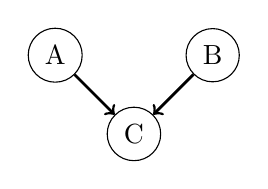
\begin{tikzpicture}
        \node[shape=circle,draw=black] (A) at (0,0) {A};
        \node[shape=circle,draw=black] (B) at (2,0) {B};
        \node[shape=circle,draw=black] (C) at (1,-1) {C};
        \path [->,line width=1pt] (A) edge node[left]{}(C);
        \path [->,line width=1pt] (B) edge node[left]{}(C);
    \end{tikzpicture}
    \end{center}

    \begin{enumerate}[label=\alph*)]
        \item Is it possible to conclude from the structure alone that $A$ and $B$ are conditionally independent given $C$? Justify your answer.\\ \\
        \noindent \textbf{Solution: } \boxed{No}, A and B are not d-separated. The path $A \rightarrow C \leftarrow B$ contains an inverted fork at node $C \in \mathcal{C}$.
        \item Suppose that the conditional distribution for $C$ is given by the following table:
        \begin{center}
        \begin{tabular}{cc|c}
            \toprule
            $A$ & $B$ & $P(C=1 \mid A,B)$ \\
            \midrule
            0 & 0 & 0.2 \\
            0 & 1 & 0.3 \\
            1 & 0 & 0.4 \\
            1 & 1 & 0.5 \\
            \bottomrule
        \end{tabular}\\
        \end{center}
        and that $P(A=1) = 0.6$ and $P(B=1) = 0.7$. Calculate $P(A=1 \mid B=1, C=1)$.\\ \\
        \noindent \textbf{Solution: } By the definition of conditional probability,
        \begin{align*}
            P(A=1\mid B=1,C=1) &= \frac{P(A=1,B=1,C=1)}{P(B=1,C=1)}\\
                        &= \frac{P(A=1,B=1,C=1)}{\sum_{a \in A}P(A=a,B=1,C=1)}
        \end{align*}
        Utilizing the graph structure,
        \begin{align*}
            P(A=1,B=1,C=1) &= P(C=1\mid A=1,B=1)\cdot P(A=1) \cdot P(B=1) = 0.21\\
            P(A=0,B=1,C=1) &= P(C=1\mid A=0,B=1)\cdot (1 -P(A=1)) \cdot P(B=1) = 0.084
        \end{align*}
        \begin{equation*}
            P(A=1\mid B=1,C=1) = \boxed{0.714}
        \end{equation*}
        \newpage
        \item Now, suppose that $P(A=1) = 0.5$, $P(B=1) = 0.5$, and $P(C=1 \mid A, B) = 0.5$ for all values of $A$ and $B$. Are $A$ and $B$ conditionally independent given $C$? Justify your answer.
        \\ \\
        \noindent \textbf{Solution: }\\From problem, $P(A=a) = P(B=b) = P(C=c \mid A=a,B=b) = 0.5\  \forall\ a \in A,\ b\in B, c \in C$. \\By the definition of conditional independence, $A$ and $B$ are conditionally independent given $C$ if and only if $P(A = a \mid B = b, C = c) = P(A = a \mid C = c)\ \forall\ a \in A, b \in B, c \in C$. \\Utilizing the graph structure,
        % ZS: This should be $P(A, B \mid C) = P(A \mid C)\cdot P(B \mid C)$.
        % ZS: I think the easiest one to verify is $P(A | B, C) = P(A \mid C)$
        \begin{equation*}
            P (A = a, B = b, C = c) = P (C = c | A = a, B = b) \cdot P (A = a) \cdot P (B = b) = 0.125
        \end{equation*}
        Marginalizing by $A$,
        \begin{align*}
            P(B=b,C=c) &= \sum_{a \in A}P(A=a,B=b,C=c)\\
            &= P(A=1,B=b,C=c) + P(A=0,B=b,C=c)\\
            &= 0.25
        \end{align*}
        By the definition of conditional probability,
        \begin{align*}
            P(A = a \mid B = b, C = c) &= \frac{P (A = a, B = b, C = c)}{P(B=b,C=c)} = 0.5
        \end{align*}
        and
        \begin{align*}
            P(A = a \mid C = c) &= \frac{\sum_{b}P (A = a, B = b, C = c)}{\sum_{b}P(B=b,C=c)}\\ 
            &= \frac{0.125 + 0.125}{0.25 + 0.25}\\
            &= 0.5
        \end{align*}
        Thus, $P(A = a \mid B = b, C = c) = P(A = a \mid C = c) = 0.5\ \forall\ a \in A, b \in B, c \in C$ so $A$ and $B$ must be conditionally independent given $C$.
    \end{enumerate}
\end{question}

\clearpage

\begin{question} (50 pts)
    Whiskers the family cat has gotten away again, however this is a fairly common occurrence, so you know that she is either in the alley (A) or at the park (P). You plan to use your camera-equipped drone to quickly search for her, however, since it is late 2024 in New Jersey, you want to avoid being sited and contributing to conspiracy theories.

\begin{itemize}[noitemsep]
    \item You must take off from home (H), and visit both sites (you do not need to account for returning home). 
    \item You seek the policy that minimizes the expected battery usage.
    \item Due to obstacles and wind the amount of battery used is not proportional to the distance, but instead is given in the table below.
    \item There is also a probability the drone encounters a person along the route given in the second table below.  Since a person may arrive or leave, the presence of a person is independent from time step to time step. If the drone encounters a person, it will return to the location it just left from but will have used the same amount of battery as if it had arrived at the desired location.
\end{itemize}

    \begin{minipage}{0.5\textwidth}
    \centering
    Battery usage table\\
        \begin{tabular}{r@{\hspace{1em}}lccc}
            \toprule
       To:     & & A & P \\
            \midrule
            & H & 1 & 2 \\
       From: & A & 0 & 1 \\
            & P & 1 & 0 \\
            \bottomrule
        \end{tabular}
    \end{minipage}
    \begin{minipage}{0.5\textwidth}
    Probability of encountering a person\\
        \begin{tabular}{r@{\hspace{1em}}lccc}
            \toprule
       To:     & & A & P \\
            \midrule
            & H &  0.3 & 0.1 \\
       From: & A &  0.0 & 0.2 \\
            & P &  0.1 & 0.0 \\
            \bottomrule
        \end{tabular}
    \end{minipage}

    \begin{enumerate}[label=\alph*)]
        \item Formulate this as a Markov decision process by writing down the state space, action space, transition probabilities, reward function. You can choose any discount factor 0.9 or above.
         \\ \\
        \noindent \textbf{Solution: }
        Let $F$ designate the finish state reached when both the park and the alley are searched.
        \begin{align*}
            S &= \{H,A,P,F\} \\
            A &= \{A,P\}\\
            \gamma &= 0.9\\
            R(s,a) &= 
            \begin{cases}
                -1& \text{ if } s\in\{H,P\}\text{ and } a = A\\
                -1& \text{ if } s = A\text{ and } a = P\\
                -2& \text{ if } s = H\text{ and } a = P\\
                % -100 & \text{ if } s = a \quad \text{(keeps the quad from staying in the same location, less than $-2/(1-\gamma)$)} \\
                0 & \text{ o.w.}
            \end{cases}\\
            T^A &= \begin{bmatrix}
                            0.3 & 0.7 & 0 & 0\\
                            1 & 0 & 0 & 0\\
                            0 & 0 & 0.1 & 0.9\\
                            0 & 0 & 0 & 1\\
                         \end{bmatrix}\\
             T^P &= \begin{bmatrix}
                            0.1 & 0 & 0.9 & 0\\
                            0 & 0.2 & 0 & 0.8\\
                            0 & 0 & 0 & 0\\
                            0 & 0 & 0 & 1\\
                         \end{bmatrix}\\
        \end{align*}
        Note that if $s = a$, the vehicle transitions back to home. Since all rewards are negative, this will prevent the vehicle from staying in the same location. There are other ways to accomplish this, for instance with a reward for reaching the finish state (this is a little more cumbersome to represent) and a large negative reward, for instance $-2/(1-\gamma)$, for staying in the same location. It is also acceptable to use the large staying penalty with only three states because it forces the vehicle to move and visit both locations.
        \item Write down the following policies as functions of the states that you defined. Make sure to define an action for every state.
        \begin{itemize}[noitemsep]
            \item Policy 1: Go to the alley first, then the park.
            \item Policy 2: Go to the park first, then the alley.
        \end{itemize}
        \textbf{Solution: }
        \begin{align*}
            \pi_1(s) &= \begin{cases}
                            A& \text{if } s=H\\
                            P&\text{o.w.}
                        \end{cases}\\
            \pi_2(s) &= \begin{cases}
                            P& \text{if } s=H\\
                            A&\text{o.w.}
                        \end{cases}\\
        \end{align*}
        \item Which of the two policies is better? Justify your answer by showing which policy will accrue the most reward. \\ \\
        \textbf{Solution: } Using the Bellman expectation equation,
        \begin{equation*}
            \vec{U}^\pi = (I - \gamma*T^\pi)^{-1}\vec{R}^\pi
        \end{equation*}
        and the following $T$ and $R$ matrices for each policy,
        \begin{align*}
            T^{\pi_1} &= \begin{bmatrix}
                            0.3 & 0.7 & 0 & 0\\
                            0 & 0.2 & 0 & 0.8\\
                            0 & 0 & 1 & 0\\
                            0 & 0 & 0 & 1\\
                         \end{bmatrix}\\
            R^{\pi_1} &= 
            \begin{bmatrix}
                -1\\
                -1\\
                0\\
                0
            \end{bmatrix}\\
             T^{\pi_2} &= \begin{bmatrix}
                            0.1 & 0 & 0.9 & 0\\
                            0 & 1 & 0 & 0\\
                            0 & 0 & 0.1 & 0.9\\
                            0 & 0 & 0 & 1\\
                         \end{bmatrix}\\
            R^{\pi_2} &= 
            \begin{bmatrix}
                -2\\
                0\\
                -1\\
                0
            \end{bmatrix}\\
        \end{align*}
        we get the following expected values for each policy.
        \begin{align*}
            U^{\pi_1} &= [-2.42,-1.22,0,0]^T\\
            U^{\pi_2} &= [-3.18,0,-1.10,0]^T
        \end{align*}
        Policy 1 has a lower expected battery cost for state $H$, so it is the better policy.
    \end{enumerate}
\end{question}

% \clearpage

% (Additional Room for Question 2)

\clearpage

\begin{question} (10 pts)
You are evaluating two MDP policies through simulation. For policy 1, you run 2000 simulations, recording the total reward, $\hat{u}$, obtained in each simulation. The sample standard deviation for this set of simulations is 50. For policy 2, you run 300 simulations, again recording the total reward of each and find that the sample standard deviation is 15. For which policy do you have a better estimate of the expected total reward, $U(\pi)$? Justify your answer.
\end{question} 
\noindent \textbf{Solution: }
Given $N_{\pi_1} = 2000$, std$(\hat{u}_{\pi_1}) = 50$, $N_{\pi_2} = 300$, and std$(\hat{u}_{\pi_2}) = 15$.
\begin{equation*}
    SEM_{\pi_i} = \frac{\text{std}(\hat{u}_{\pi_i})}{\sqrt{N_{\pi_i}}}
\end{equation*}
Calculating the standard error of the mean, $SEM_{\pi_1} \approx 1.12$, $SEM_{\pi_2} \approx 0.866$. Since $SEM_{\pi_1} > SEM_{\pi_2}$, we have a better estimate of $\boxed{U(\pi_2)}$.

\vspace{10cm}

\begin{question} (10 pts)
Consider an MDP with states that are integers. Policy $\pi_1$ has value $U^{\pi_1}(1) = 10.0$ and $U^{\pi_1}(2) = 12.0$. Policy $\pi_2$ has value $U^{\pi_2}(1) = 11.0$ and $U^{\pi_2}(2) = 10.0$. Is it possible that either one of these policies is an optimal policy? Justify your answer.
\end{question}
\noindent \textbf{Solution: }
Since the Bellman operator is a contraction mapping, $U^*$ is unique and an optimal policy will have $U^{\pi^*}(s) = U^*(s)$ for all states. $U^*(s) \geq U^\pi(s)$ for all policies $\pi$. Since $U^{\pi_1}(1) < U^{\pi_2}(1) \leq U^*(1)$, $\pi_1$ is not optimal. Similarly, since $U^{\pi_2}(2) < U^{\pi_1}(2) \leq U^*(2)$, $\pi_2$ is not optimal.
% An optimal policy should maximize the expected sum of future rewards (Q) for any state. Because policy 1 has a higher utility for state 1, but a lower utility than policy 2 for state 2, neither policy is maximizing the expected sum of future rewards for both of the given states, and thus neither policy can be optimal.
\end{document}
